% Preamble
\documentclass[linenumbers]{aastex631}
%\documentclass[twocolumn, linenumbers, twocolappendix]{aastex631}
%\documentclass[twocolumn]{aastex631}
\usepackage{natbib}
\usepackage{latexsym}
\usepackage{graphicx}
\usepackage{epsfig}
\usepackage{amssymb}
\usepackage{amsmath}
\usepackage{epstopdf}
\usepackage{hyperref}
\usepackage{xcolor}

%%%% Custom commands
\newcommand{\yL}{\ensuremath{\mathcal{Y}_{\rm{L}}}}
\newcommand{\yS}{\ensuremath{\mathcal{Y}_{\rm{S}}}}
\newcommand{\justgrad}{\ensuremath{\nabla}}
\newcommand{\gradrad}{\ensuremath{\nabla_{\rm{rad}}}}
\newcommand{\gradad}{\ensuremath{\nabla_{\rm{ad}}}}
\newcommand{\gradC}{\ensuremath{\nabla_{\mathrm{C}}}}
\newcommand{\gradmu}{\ensuremath{\nabla_{\mu}}}
\newcommand{\gradL}{\ensuremath{\nabla_{\mathrm{L}}}}
\newcommand{\gradT}{\ensuremath{\nabla_{\mathrm{T}}}}
\newcommand{\Ro}{\ensuremath{\mathrm{R}_{0}}}
\newcommand{\delp}{\ensuremath{\delta_{\rm{p}}}}
\newcommand{\Fbot}{\ensuremath{F_{\rm{bot}}}}
\newcommand{\Ftot}{\ensuremath{F_{\rm{tot}}}}
\newcommand{\Frad}{\ensuremath{F_{\rm{rad}}}}
\newcommand{\Fconv}{\ensuremath{F_{\rm{conv}}}}
\newcommand{\Fcz}{\ensuremath{F_{\rm{cz}}}}
\newcommand{\mP}{\ensuremath{\mathcal{P}}}
\newcommand{\mD}{\ensuremath{\mathcal{D}}}
\newcommand{\dP}{\ensuremath{\delta_{\rm{p}}}}
\newcommand{\Lcz}{\ensuremath{L_{\rm{CZ}}}}
\newcommand{\mR}{\ensuremath{\mathcal{R}}}
\newcommand{\mS}{\ensuremath{\mathcal{S}}}
\newcommand\Pran{\ensuremath{\mathrm{Pr}}}
\newcommand{\brunt}{{Brunt-V\"{a}is\"{a}l\"{a}}}

\newcommand{\angles}[1]{\langle #1 \rangle}
\newcommand{\pd}[1]{\partial_{#1}}
\renewcommand{\vec}[1]{\boldsymbol{#1}}
\newcommand{\M}[1]{\mathbf{#1}}
\renewcommand{\dot}{\vec{\cdot}}
\renewcommand{\bar}[1]{\overline{#1}}
\newcommand{\grad}{\vec{\nabla}}
\newcommand{\cross}{\vec{\times}}
\newcommand{\laplacian}{\nabla^2}

\newcommand{\editone}[1]{\textcolor{orange}{#1}}

\newcommand{\todo}[1]{ {\color{blue} \noindent\footnotesize \\\textsf{}TODO:} \textsf{#1}\\\noindent }


%%%% Journal preamble
\received{}
\revised{}
\accepted{}
\published{}
\submitjournal{RNAAS}

\shorttitle{CBM Processes \& Structure}
\shortauthors{Anders et al}


\begin{document}

%%%% Title and Abstract
\title{The Processes and Structure of Convective Boundary Mixing}
\author[0000-0002-3433-4733]{Evan H. Anders}
\affiliation{CIERA, Northwestern University, Evanston IL 60201, USA}
\author[0000-0001-5048-9973]{Adam S. Jermyn}
\affiliation{Center for Computational Astrophysics, Flatiron Institute, New York, NY 10010, USA}
\author[0000-0002-7635-9728]{Daniel Lecoanet}
\affiliation{CIERA, Northwestern University, Evanston IL 60201, USA}
\affiliation{Department of Engineering Sciences and Applied Mathematics, Northwestern University, Evanston IL 60208, USA}
\author[0000-0003-2124-9764]{J. R. Fuentes}
\affiliation{Department of Physics and McGill Space Institute, McGill University, 3600 rue University, Montreal, QC H3A 2T8, Canada}
\author[0000-0002-0963-4881]{Lydia Korre}
\affiliation{Laboratory for Atmospheric and Space Physics, Boulder, CO 80303, US}
\author[0000-0001-8935-219X]{Benjamin P. Brown}
\affiliation{Laboratory for Atmospheric and Space Physics, Boulder, CO 80303, US}
\affiliation{University of Colorado Department of Astrophysical and Planetary Sciences, Boulder, Colorado 80309, USA}
\author[0000-0001-8531-6570]{Jeffrey S. Oishi}
\affiliation{Bates College Department of Physics and Astronomy, Lewiston, Maine 04240, USA}

\correspondingauthor{Evan H. Anders}
\email{evan.anders@northwestern.edu}

\begin{abstract}
    Convective motions extend beyond the nominal boundaries of a convection zone.
    The mechanisms which drive these motions are collectively called ``convective boundary mixing'' (CBM).
    In this note, we discuss three fluid dynamical processes: mechanical overshoot, entrainment, and penetrative convection.
    We describe the structure of a convective boundary when all of these processes are active.
    To resolve discrepancies between models and observations, the stellar astrophysics community must distinguish between these processes and parameterize each of them separately in 1D evolutionary models.
\end{abstract}
\keywords{Stellar convection zones (301), Stellar physics (1621); Stellar evolutionary models (2046)}


%%%% Body of paper
\section{Introduction}
\label{sec:introduction}
Observations tell us that we do not understand convective boundary mixing (CBM).
\todo{CITE}
In order to resolve this problem, we need to build a community understanding of CBM processes.
In this note, we will briefly describe three fluid dynamical processes: convective overshoot, entrainment, and convective penetration.
Each of these processes likely occurs at convective boundaries in stars, and each should be separately parameterized and employed in 1D stellar evolution models.


\begin{figure*}[t!]
\centering
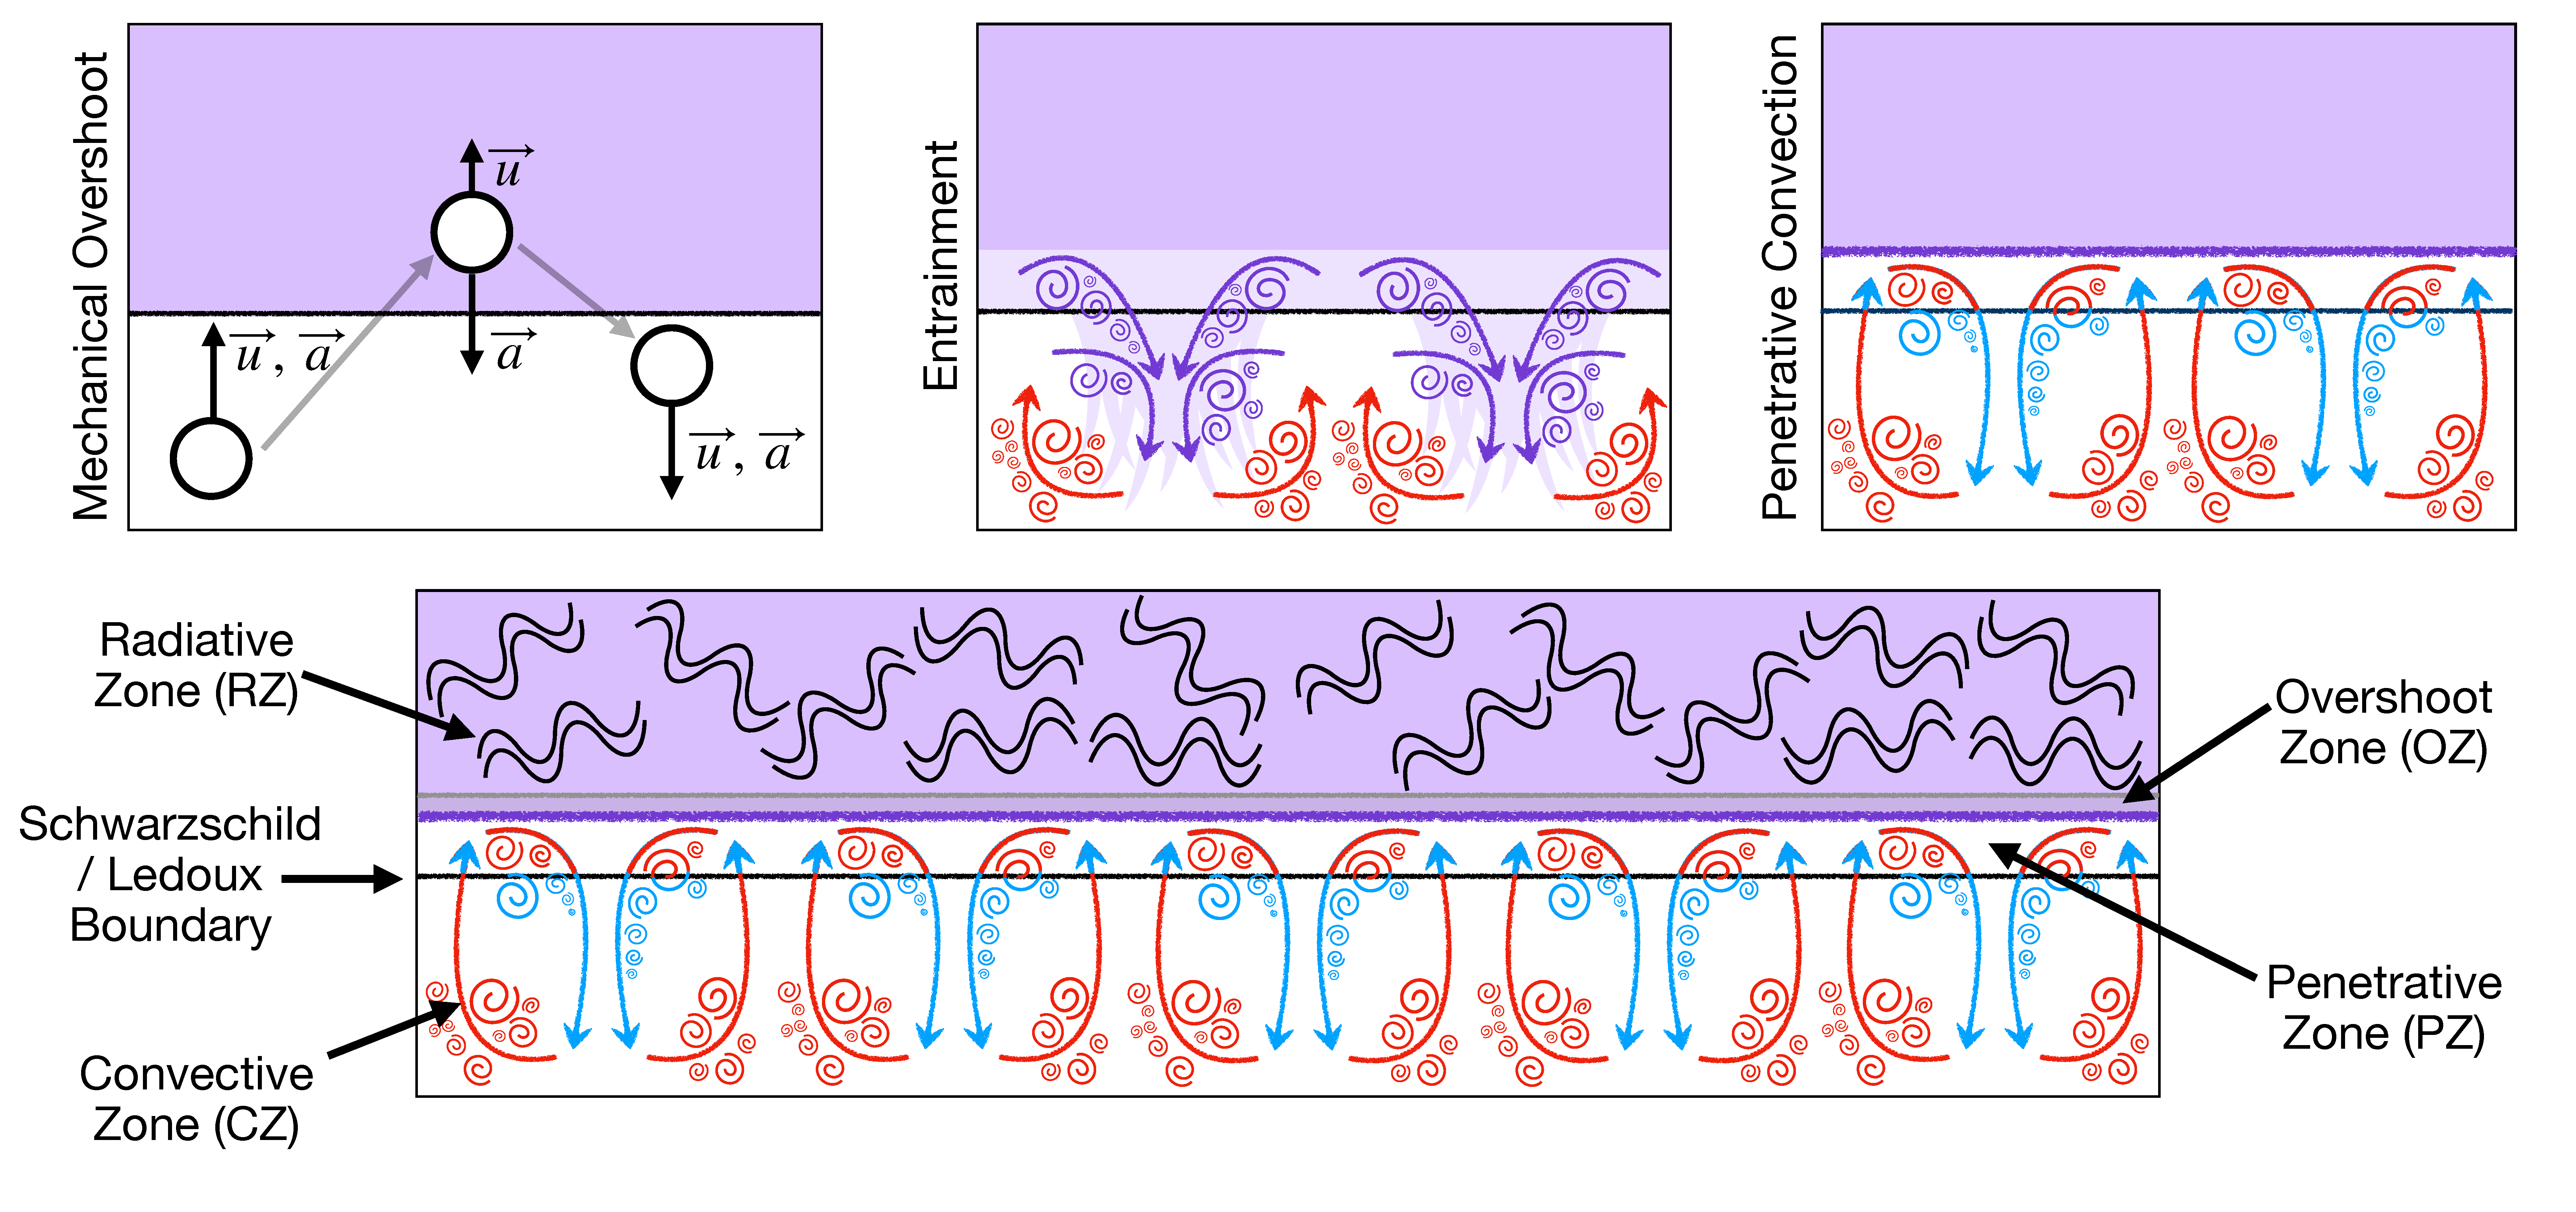
\includegraphics[width=\textwidth]{processes_and_structure_figure.pdf}
\caption{
    The three processes discussed in Sec.~\ref{sec:processes} are schematically demonstrated in the top row.
    White fluid has the properties of the well-mixed convective zone (CZ), while purple fluid is stable.
    (Left) Mechanical overshoot occurs when a fluid parcel from the CZ crosses into the radiative zone (RZ); since its properties differ from those of the stable background, it is accelerated back into the CZ.
    (Middle) Motions generated by overshooting fluid parcels drag fluid from the RZ into the CZ in a process called entrainment.
    (Right) If a region of fluid beyond the convective boundary becomes well-mixed, it is a penetrative zone (PZ); divergences in the radiative flux make hot upflows turn cold and make downflows hot in this region.
    In the bottom panel, we show the structure of a statistically-stationary convective boundary.
    The CZ sits below a well-mixed PZ.
    Above the PZ, the fluid is stable but there is a small overshoot zone (OZ) where mechanical overshoot occurs.
    Above this region is the stable RZ where there are internal gravity waves excited by the convection.
\label{fig:schema}
}
\end{figure*}


\section{Convective Boundary Mixing Processes}
\label{sec:processes}

Observations make it clear that convective boundary mixing prescriptions in 1D stellar models require improvement \citep{pinsonneault_1997, claret_torres_2018, pedersen_etal_2021}.
In this section, we briefly describe three distinct processes: convective overshoot, entrainment, and penetrative convection.
In the following discussion, ``convective boundary'' refers to the location of the sign change of either the Schwarzschild or Ledoux discriminant.
In this discussion, we depict a convection zone (CZ) below an radiative zone (RZ), as in a massive star core, but these processes all occur if the picture is flipped upside-down, as in the base of the solar convection zone.

\subsection{Convective Overshoot}
Convective overshoot (or mechanical overshoot) occurs because the convective boundary is not the location where convective velocities are zero, but rather the location where the \emph{buoyant acceleration} of the fluid is zero.
The process of convective overshoot is shown in the upper left panel of Fig.~\ref{fig:schema}, where motions from the white CZ overshoot into the purple stable RZ.
Flows buoyantly decelerate beyond the convective boundary, so there is an extended overshoot zone (OZ) with nonzero convective velocities.

A simple $\Delta x = u \Delta t$ argument provides an estimate for how far convective motions overshoot.
Here $\Delta x$ is the overshoot distance, $u$ is the convective velocity, and $\Delta t \approx N^{-1}$ where $N$ is the \brunt$\,$frequency in the stable region.
There is disagreement regarding precisely how to calculate $\Delta x$, but this gives the proper flavor and shows that $\Delta x \ll H_P$ in stellar environments, where $H_P$ is the pressure scale height.

The exponential overshoot parameterization \citep[per e.g.,][]{herwig_2000} which is frequently implemented in 1D models describes this process fairly well.
However, 1D models generally treat $\Delta x$ as a free parameter, and the values needed to match observations have $\Delta x/H_P \sim \mathcal{O}(0.1)$, which is much larger than hydrodynamical simulations suggest should happen when low Mach number flows encounter very stable interfaces \citep{korre_etal_2019}.

\begin{figure*}[t]
\centering
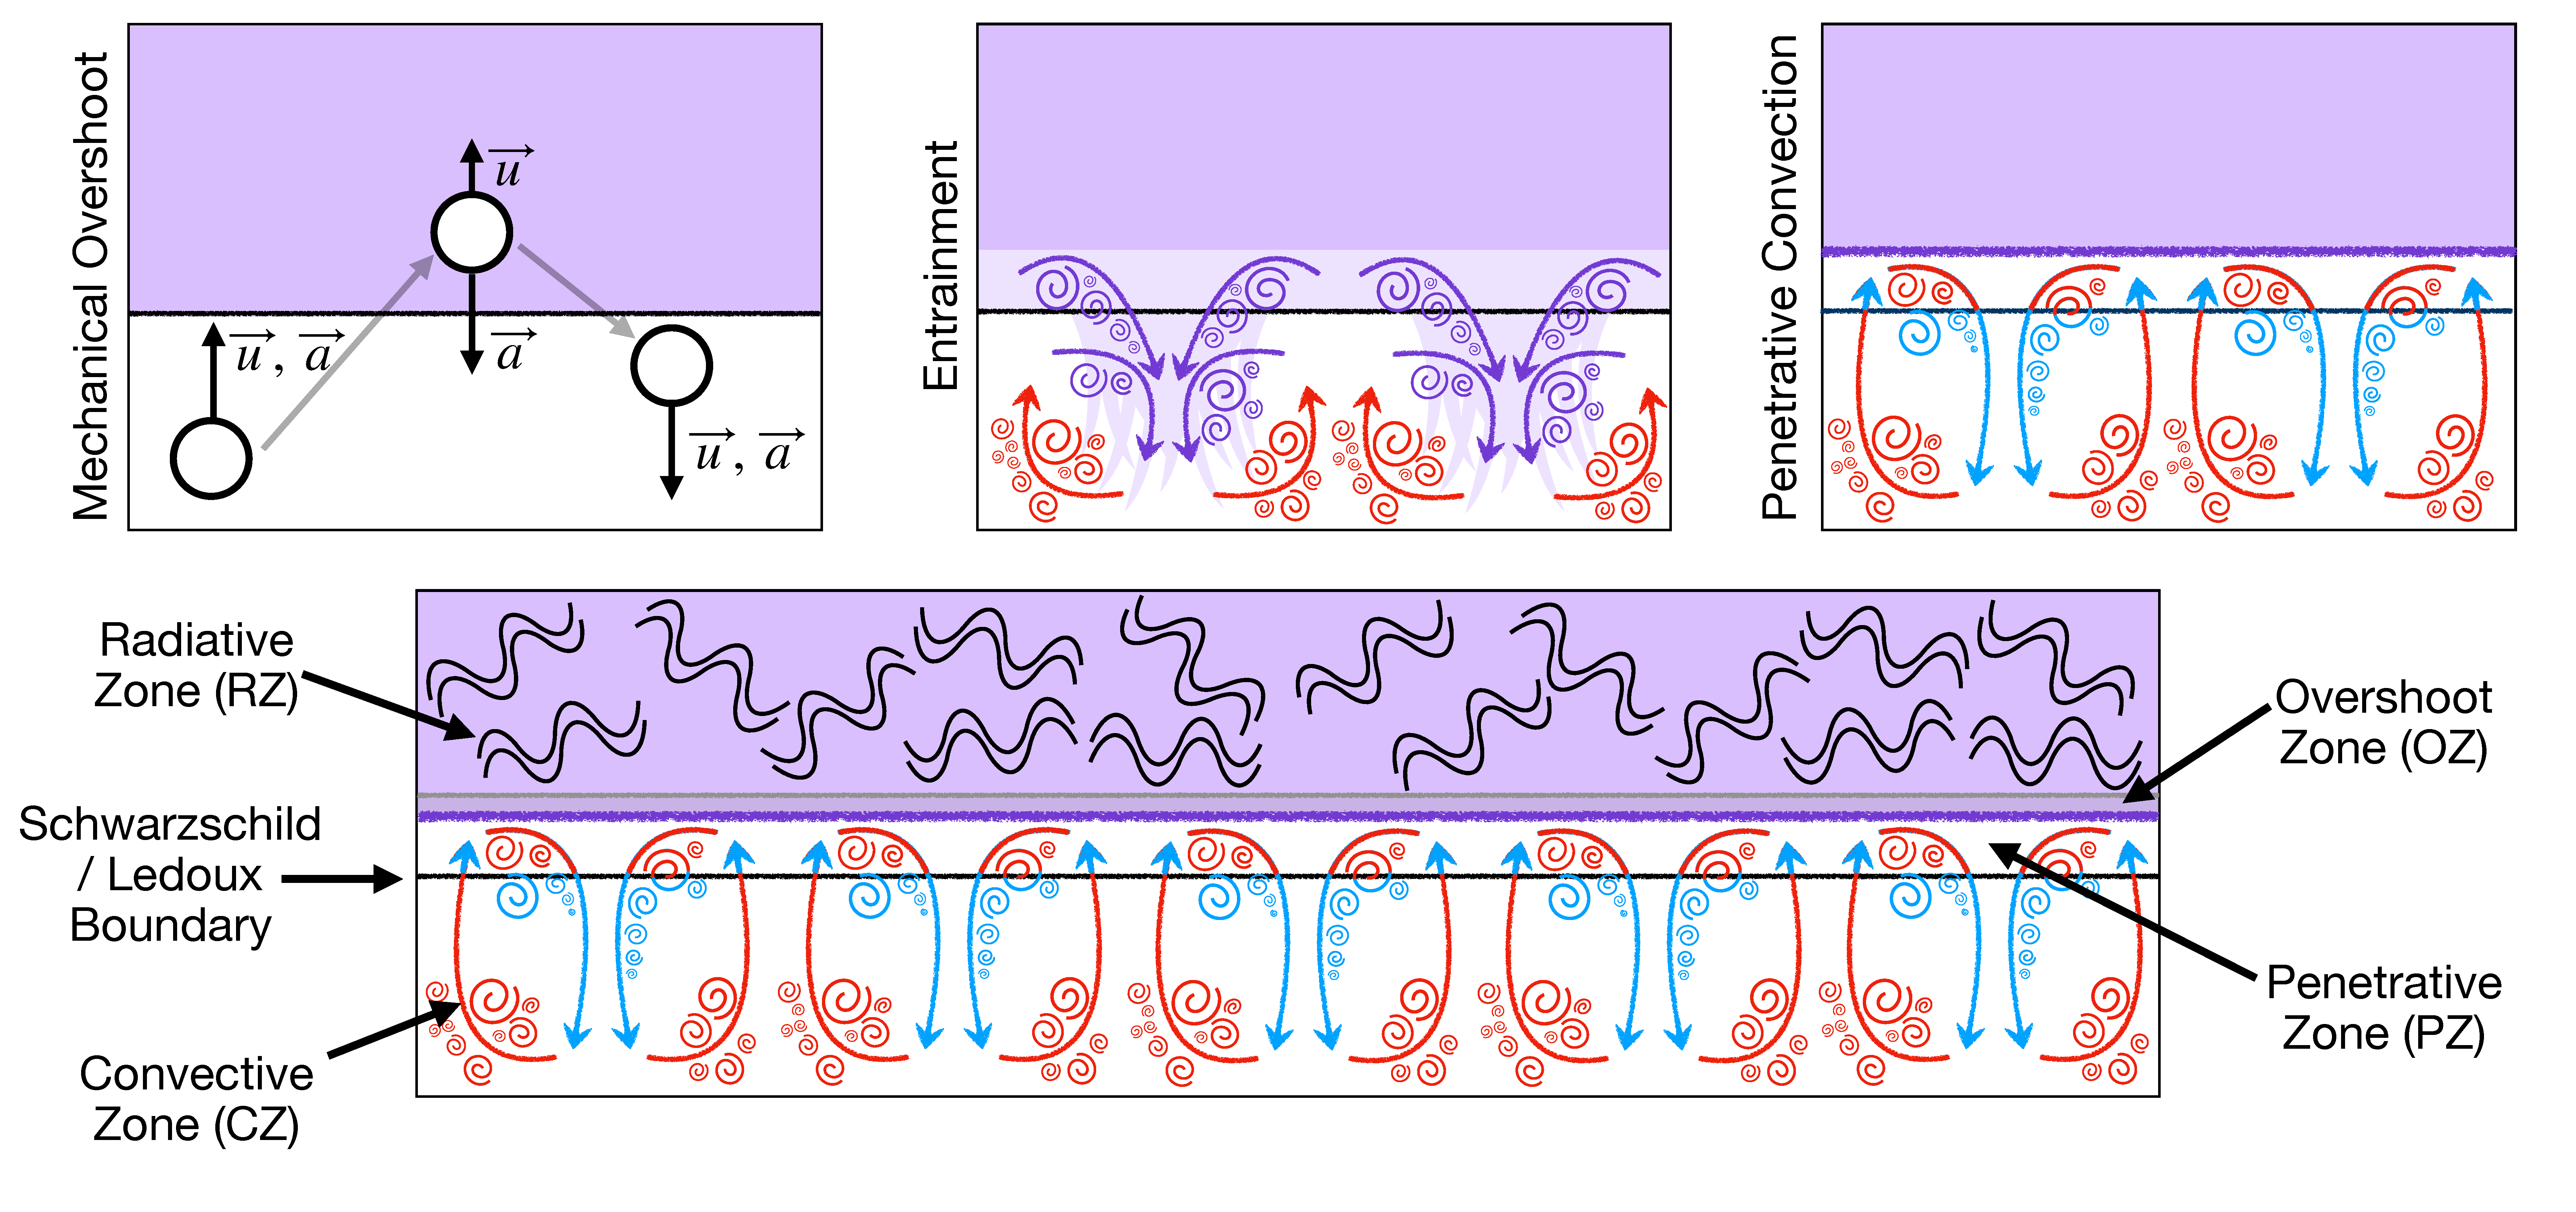
\includegraphics[width=\textwidth]{processes_and_structure_figure.pdf}
\caption{
    The three processes discussed in Sec.~\ref{sec:processes} are shown schematically in the top row.
    White fluid has the properties of the well-mixed CZ, while purple fluid is the stable RZ.
    (Left) Convective overshoot occurs when a fluid parcel from the CZ crosses into the RZ; due to a strong positive entropy gradient in the RZ, the parcel is accelerated back into the CZ.
    (Middle) Motions generated by overshooting fluid parcels drag fluid from the RZ into the CZ in a process called entrainment.
    (Right) If a region of fluid beyond the convective boundary becomes well-mixed by entrainment, it is a PZ; a non-zero divergence of the radiative flux acts as an internal cooling term, changing the buoyant signature of both upflows and downflows.
    In the bottom panel, we show the structure of a statistically-stationary convective boundary.
    The CZ sits below a well-mixed PZ.
    Above the PZ, the fluid is stable but there is a small OZ where convective overshoot occurs.
    Above this region is the stable RZ where there are internal gravity waves excited by the convection.
\label{fig:schema}
}
\end{figure*}





\subsection{Entrainment}
The process of entrainment is shown in the upper middle panel of Fig.~\ref{fig:schema}.
Return flows from overshooting convection carry fluid with the chemical and thermodynamic signature of the RZ.
This material then rapidly mixes in the CZ.
As a result, convective motions which overshoot and entrain materials can gradually move convective boundaries.
Since entrainment is linked to convective overshooting, the overshoot distance $\Delta x$ directly relates to the \emph{rate} of entrainment; this can be inferred from entrainment rate laws \citep{meakin_arnett_2007} or interface flux arguments \citep{fuentes_cumming_2020}.

Entrainment has been modeled in 1D stellar evolution software instruments by \citet{staritsin_2013} and \citet{scott_etal_2021}, but their implementations differ from one another and entrainment is not standard in any instrument.


\subsection{Penetrative Convection}
The process of penetrative convection is shown in the upper right panel of Fig.~\ref{fig:schema}.
Through continual overshoot and entrainment, convection creates well-mixed regions beyond the convective boundary \citep{anders_etal_2022}.
These well-mixed extensions of the CZ are known as penetration zones (PZs).
Since PZs grow gradually over many dynamical times, they can extend well beyond the overshoot distance $\Delta x$.

Penetrative convection most closely resembles the ``step overshoot'' prescription employed in 1D models, but penetrative convection mixes both entropy and composition.


\section{Convective Boundary Structure}
\label{sec:structure}
The structure of a convective boundary in steady state is shown in the bottom panel of Fig.~\ref{fig:schema}.
The convective boundary as determined by the Schwarzschild or Ledoux criterion is denoted by a black horizontal line, and the CZ is below that line.
In the CZ, upflows are hot and downflows are cold.
A well-mixed PZ is above the CZ.
In the PZ, the radiative luminosity exceeds the system luminosity, so the convective luminosity is negative resulting in cold upflows and warm downflows.
Both entropy and composition are mixed throughout the CZ and PZ.
The upper boundary of the PZ is marked by a purple line.
Above the PZ, there is a stably-stratified OZ where composition is mixed and a strong positive entropy gradient rapidly decelerates convective motions.
A thin grey line denotes the top of the OZ.
Above the OZ is an RZ filled with internal gravity waves.
In a statistically-stationary state, entrainment is negligible.
Entrainment is a process that reconfigures a convective boundary to create the picture in Fig.~\ref{fig:schema}, but since it is a transient process there is no ``entrainment zone.''


\section{Conclusion}
\label{sec:conclusions}
Convective boundary mixing (CBM) is a conglomeration of a few distinct dynamical processes.
These processes include convective overshoot, entrainment, and penetrative convection.
A thorough understanding and parameterization of each of these processes can reduce discrepancies between models and observations.

We have not made any distinction between radiative zones which are \emph{thermally} stable and those which are \emph{compositionally} stable.
Composition gradients are subject to the processes discussed in this work in the same way as thermal gradients.
The only distinction is that the radiative flux, and divergences in it, act to restore the thermal gradients to their radiative values, while composition gradients have no restoring flux.

Modeling of convective boundaries has plagued stellar structure modelers for many years \citep{mesa1, mesa4, mesa5}.
Unfortunately, throughout the stellar structure literature, ``convective overshoot'', ``convective penetration'', and ``convective boundary mixing'' are often used interchangeably, which increases confusion regarding this complex topic.
By reaching community agreement on both the \emph{terminology} of convective boundary mixing and the \emph{processes} that terminology refers to, we can better identify where models behave poorly and design experiments to improve them.




\bibliographystyle{aasjournal}
\bibliography{biblio}
\end{document}
